
\section{Bedienoberfläche}

Hier sollen die Skizzen/Prototypen von Bedienoberflächen dargestellt werden, als auch die Zusammenhänge zwischen denen (wie gelingt man von einem zu dem anderen Fenster/Ansicht). Ein Beispiel für Bildereinbau in LaTeX ist die Abbildung~\ref{gui:zusammenhang}.\footnote{Bevor Sie mit den Skizzen anfangen, überlegen Sie sich, welche virtuelle Räume im System zu haben sind und dann halte Sie die Namen der GUI-Fenstern mit diesen konsistent.}

\newcounter{gui}\setcounter{gui}{10}

\begin{description}[leftmargin=5em, style=sameline]	
	\begin{lhp}{gui}{GUI}{gui:beispiel}
		\item[Name:] Vorraum-Interface
		\item[Beschreibung:] Interface für Anmeldung
		\item[Relevante Systemfunktionen:] \ref{funk:zugriff}
		\item[Abbildungen:] \ref{gui:login}
	\end{lhp}
\end{description}

\begin{description}[leftmargin=5em, style=sameline]	
	\begin{lhp}{gui}{GUI}{gui:beispiel}
		\item[Name:] Zusammenhänge
		\item[Beschreibung:] Zusammenhänge zwischen GUI-Ansichten
		\item[Relevante Systemfunktionen:] Alle
		\item[Abbildungen:] \ref{gui:zusammenhang}
	\end{lhp}
\end{description}

\begin{figure}
	\centering
	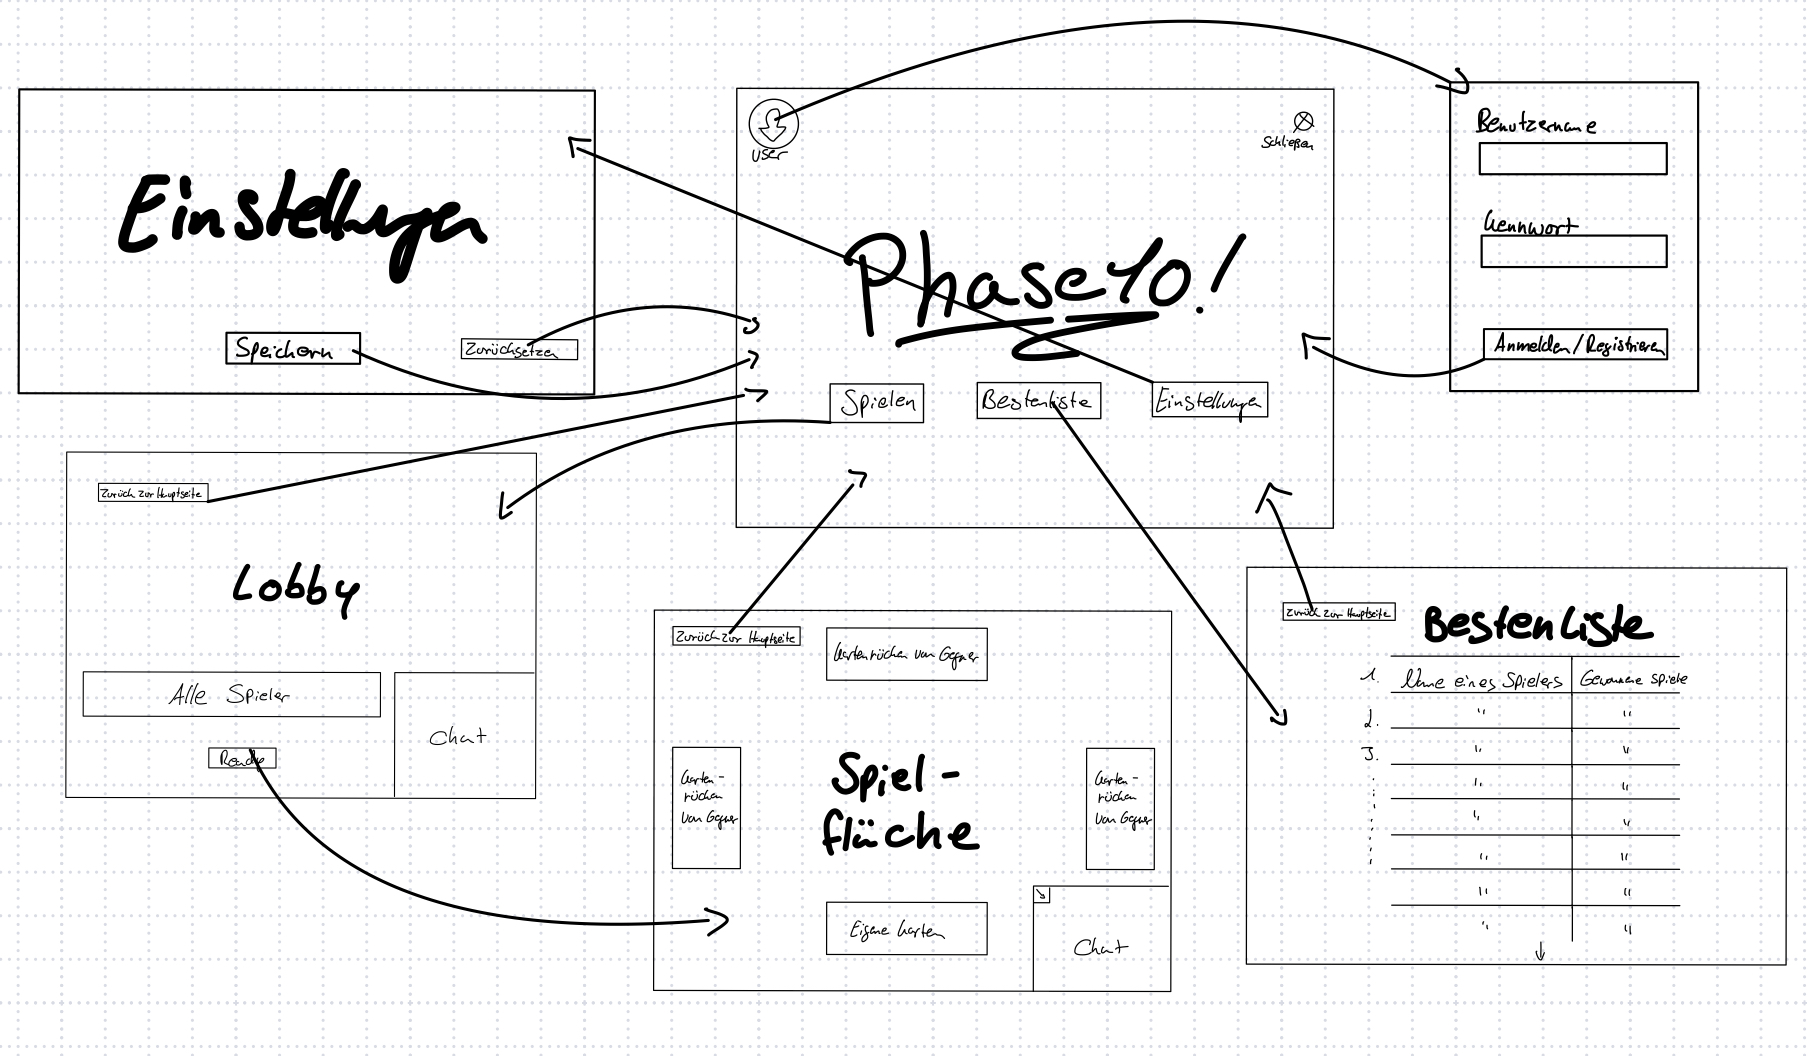
\includegraphics[width=0.9\textwidth]{img/gui-zusammenhang}
	\caption{Beispiel zur Darstellung der Zusammenhänge zwischen GUI-Ansichten.}
	\label{gui:zusammenhang}
\end{figure}

\begin{figure}
	\centering
	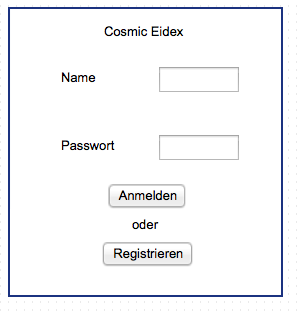
\includegraphics{img/gui-einloggen}
	\caption{Beispiel für ein GUI-Mockup. Dieser Text ist auch nur ein Beispiel :)}
	\label{gui:login}
\end{figure}